\documentclass[11pt]{article}

\usepackage[margin=1in]{geometry}
\usepackage{booktabs}
\usepackage{graphicx}
\usepackage{hyperref}
\usepackage{tabularx}
\usepackage{xcolor}

\hypersetup{
  colorlinks=true,
  linkcolor=blue!55!black,
  citecolor=blue!55!black,
  urlcolor=blue!55!black
}

\title{Bubble Dynamics Research Tools: A Living Catalog of Open Data, Code, and Models for Boiling and Multiphase Bubble Analysis}

\author{Bubble Dynamics Research Tools Maintainers\\
\small University of Arkansas NED3 community catalog\\
\small \texttt{https://github.com/UARK-NED3/Bubble-Dynamics-Research-Tools}}

\date{Draft: July 20, 2026}

\begin{document}
\maketitle

\begin{abstract}
Bubble-dynamics research increasingly depends on reusable computational and data resources: high-speed-video segmentation tools, acoustic and acoustic-emission sequence models, thermal-label datasets, interface-resolved solvers, reduced-order bubble models, and scientific machine-learning benchmarks. These resources are scattered across repositories, data archives, institutional pages, and papers, which makes it difficult for new users to identify appropriate tools or for experienced users to track emerging methods such as Bubbleformer. This paper describes \emph{Bubble Dynamics Research Tools}, a living catalog that organizes open resources for boiling vapor bubbles, gas-liquid bubbles, cavitation-like dynamics, and adjacent multiphase-flow analysis. The July 2026 snapshot contains 55 cataloged entries, represented in a machine-readable CSV table and rendered into user-facing summaries, a workflow starter matrix, workflow-oriented quick picks, a reproducibility audit, metadata-coverage dashboards, blocker-oriented maintenance frontiers, reduced-order starter-path and triage tables, dataset adoption ladders, and reproducible figures. The catalog shows a shift from isolated image-processing scripts toward multimodal datasets, segmentation-and-tracking pipelines, acoustic heat-flux models, and simulation benchmarks for long-horizon forecasting and compressible multiphase simulation. We describe the curation protocol, metadata schema, evidence-oriented summary visualizations, example user workflows, and limitations of interpreting a curated catalog as a literature census. The repository is designed as a maintainable research infrastructure artifact: new entries can be screened, added to the source table, and propagated to documentation and figures through a single rendering script.
\end{abstract}

\section{Introduction}

Bubble dynamics sits at the intersection of heat transfer, multiphase flow, imaging, acoustics, and numerical simulation. In boiling systems, bubble nucleation, growth, coalescence, departure, and dryout shape heat-transfer performance and critical heat-flux risk. In broader gas-liquid systems, bubble rise, bursting, cavitation, and coalescence determine transport, mixing, and interfacial exchange. The field has therefore moved from manual inspection of a few representative images toward computational pipelines that can extract bubble statistics, infer heat flux, classify regimes, and forecast multiphase dynamics.

This tool-driven shift creates a practical problem. Researchers can now choose among specialized boiling image frameworks such as BubbleID \cite{dunlap2024bubbleid}, acoustic and acoustic-emission regression workflows such as SeqReg and Hit2Flux \cite{dunlap2023acoustic,dunlap2025hit2flux}, simulation datasets such as BubbleML \cite{hassan2023bubbleml}, forecasting models such as Bubbleformer \cite{hassan2025bubbleformer}, compressible multiphase solvers such as MFC \cite{wilfong2026mfc}, and general utilities such as scikit-image \cite{vanderwalt2014scikitimage}, Trackpy \cite{allan2024trackpy}, and napari \cite{sofroniew2024napari}. New resources appear quickly, while older resources may become archived, renamed, or superseded. A static README can become stale even when it was carefully curated at the time of writing.

The \emph{Bubble Dynamics Research Tools} repository addresses this problem by treating the catalog itself as a reproducible research artifact. The core contribution is not a new segmentation model or CFD solver; it is a structured map of reusable resources, a lightweight curation protocol, and scripts that keep tables and figures synchronized with the source data. This paper documents the July 2026 snapshot of the catalog and explains how the repository can be used and maintained.

\section{Repository Scope}

The repository includes resources that support at least one practical bubble-dynamics workflow:
\begin{itemize}
  \item extract bubble shape, centroid, diameter, departure, coalescence, interface velocity, vapor fraction, or related image-derived metrics;
  \item analyze hydrophone, microphone, acoustic-emission, or thermal signals associated with boiling or bubble events;
  \item estimate heat flux, regime, critical-heat-flux proximity, or thermal state from synchronized measurements;
  \item simulate bubbles, droplets, foams, cavitation-like oscillations, or interface-resolved multiphase flows;
  \item train, benchmark, or validate machine-learning and scientific-machine-learning models on bubble or boiling dynamics.
\end{itemize}

The catalog intentionally includes both domain-specific tools and adjacent utilities. A pool-boiling image framework is directly relevant, but so is a mature image-labeling tool when a user needs to create new annotations. Similarly, CFD solvers and reduced-order Rayleigh-Plesset-style codes are included because they provide reference calculations and simulation infrastructure even when they are not packaged as boiling-analysis applications. Name-collision resources are listed separately when a similarly named project could confuse users.

\section{Curation Protocol and Metadata}

The source of truth is the file \texttt{data/resources.csv}. Each row represents a resource and includes the fields summarized in Table~\ref{tab:schema}. The schema is intentionally simple so that it can be edited in a spreadsheet, rendered by a short Python script, and reviewed in a pull request.

\begin{table}[t]
\centering
\caption{Core metadata fields used in the catalog.}
\label{tab:schema}
\begin{tabularx}{\linewidth}{@{}lX@{}}
\toprule
Field & Purpose \\
\midrule
\texttt{name}, \texttt{id}, \texttt{url} & Human-readable name, stable row identifier, and primary link. \\
\texttt{kind} & Resource type, such as code, dataset, utility, model artifact, example, or documentation. \\
\texttt{category} & Workflow grouping, such as optical imaging, acoustics, SciML, CFD, or reduced-order dynamics. \\
\texttt{regime} & Physical regime or intended use, such as pool boiling, subcooled flow boiling, bubble bursting, or gas-solid fluidized beds. \\
\texttt{modality} & Inputs or data products, including images, masks, hydrophone signals, AE hits, CFD fields, ODE states, and thermal data. \\
\texttt{workflow} & What a user can do with the resource. \\
\texttt{stack} & Primary software stack, archive type, or solver family. \\
\texttt{year}, \texttt{status}, \texttt{license} & Resource year, maintenance status, and license or archive-term note. \\
\texttt{source\_checked} & Date of the most recent manual inspection. \\
\bottomrule
\end{tabularx}
\end{table}

Candidate resources are screened before entry. The maintainer checks whether the resource provides reusable code, data, model weights, examples, or documentation; whether the physical regime is relevant to bubble dynamics or a necessary adjacent workflow; whether the license or archive terms are visible; and whether the README or associated paper gives enough information to understand inputs, outputs, assumptions, and limitations. This is especially important for AI/ML tools because performance in one apparatus, fluid, surface, or simulation family does not imply generalization to another. To keep these signals visible after entry, the repository now generates a reproducibility-audit page that groups resources by evidence bundle (for example, code plus data plus paper versus partial link coverage), flags manual-review priorities such as generic license labels or review-sharing links, summarizes direct-paper-link coverage, citation-evidence coverage, and license clarity by category, counts the remaining backlog by review-focus type, cross-tabs that backlog by workflow category, distinguishes blocker type (maintainer backfill versus citation discoverability versus genuine upstream sparsity versus unstable access links), adds both category-level blocker and paper-evidence figures, ranks both a general maintenance frontier and a filtered backfill-ready queue by combined issue count, category concentration, verification age, and scope alignment, and now also renders dataset and reduced-order adoption ladders plus workflow- and reduced-order-specific starter matrices so repeated critiques are converted into explicit user guidance rather than left as maintainer-only debt accounting. The June 22 through July 20 revisions backfill canonical software citations for core utilities and solver infrastructure such as scikit-image \cite{vanderwalt2014scikitimage}, Trackpy \cite{allan2024trackpy}, napari \cite{sofroniew2024napari}, Fiji \cite{schindelin2012fiji}, PIVlab \cite{thielicke2021pivlab}, Basilisk \cite{popinet2009basilisk}, and OpenFOAM \cite{jasak2007openfoam}, recover scholarly links plus verified MIT licenses for previously under-documented optical/computer-vision entries such as BubbleNet \cite{zhai2022bubblenet}, BubMask \cite{kim2021bubmask}, and FluidNexus \cite{gao2025fluidnexus}, clarify that the `sound of boiling` Mendeley dataset is released under CC BY 4.0 with DOI-level metadata even though its associated paper link remains absent from the public archive page, close the `Results of bubble detection and tracking of subcooled boiling flow` archive row with a verified CC BY 4.0 license plus the linked 2025 thermal-hydraulic analysis paper, backfill the explicit `cc-by-nc-4.0` license exposed on the FluidVerse shock-bubble dataset card, treat documentation pages and thesis-style research repositories differently from ordinary metadata-transfer rows, correct a second-order ranking problem in which peripheral transfer-only rows could still dominate the maintainer frontier, separate title-level citation verification from genuinely missing paper evidence, add reduced-order triage tables so pedagogical or prototype single-bubble solvers are no longer conflated with the small set of reference-backed reduced-order anchors, add a dataset adoption ladder so archive-backed benchmarks are separated from citation-verified or archive-only leads before users cite or download them, and add both a workflow starter matrix and a reduced-order starter-path matrix so users no longer need to infer their first tool choice by mentally merging quick picks, category counts, and audit tables. The July 20 pass especially targeted the next repeated reduced-order critique by adding the explicitly licensed APECSS cavitation-bubble package as a source-verified anchor, upgrading the Harvard Dataverse multimodal boiling dataset to a direct-paper row through its Data in Brief article, and converting both kozakaron sonochemistry repositories from `no paper evidence` backlog into paper-backed but still license-unclear entries. Just as importantly, the audit now distinguishes standard open or permissive licenses from explicit but restrictive Creative Commons or source-available terms, which prevents technically strong resources such as NUCLEUS, FluidVerse, and FluidX3D \cite{feeney2026nucleusmoe,lehmann2021fluidx3d} from being overstated as open for downstream reuse.

\section{June 2026 Catalog Snapshot}

The July 2026 snapshot contains 55 resources, of which 54 are directly usable or adjacent technical resources and one is a name-collision warning. Figure~\ref{fig:category} summarizes the distribution of entries by workflow category. Datasets, optical imaging/computer vision tools, and CFD or multiphase simulation resources form the largest groups. This distribution reflects the current practical needs of the field: researchers often require both measurement data and analysis software, while simulation tools remain central for controlled studies and SciML benchmarks.

\begin{figure}[t]
\centering
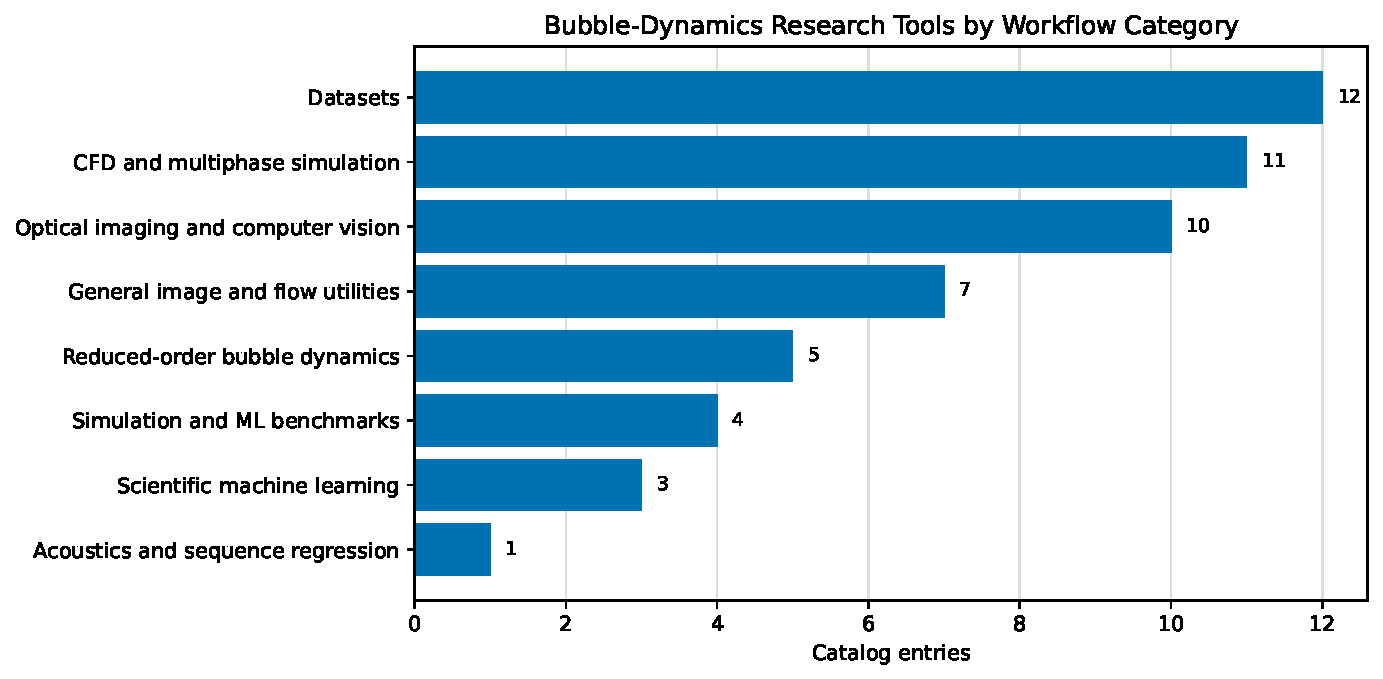
\includegraphics[width=0.92\linewidth]{figures/resource_category_summary.pdf}
\caption{Catalog entries by workflow category. Counts describe the curated repository snapshot, not the full literature.}
\label{fig:category}
\end{figure}

The time distribution in Fig.~\ref{fig:timeline} highlights a recent increase in open datasets, image-analysis workflows, and scientific-machine-learning benchmarks. Older entries are dominated by established solver and utility infrastructure. Recent entries include BubbleID for pool-boiling image analysis \cite{dunlap2024bubbleid}, VideoSAM for high-speed-video phase segmentation \cite{maduabuchi2024videosam}, Zhou and co-workers' subcooled-flow-boiling detection and tracking resources \cite{zhou2024subcooled,zhou2025thermalhydraulic}, BubbleML and BubbleML 2.0 \cite{hassan2023bubbleml,hassan2025bubbleformer}, NUCLEUS for unified multi-fluid surrogate modeling \cite{feeney2026nucleusmoe}, and MFC for compressible bubbly and cavitating multiphase simulation \cite{wilfong2026mfc}.

\begin{figure}[t]
\centering
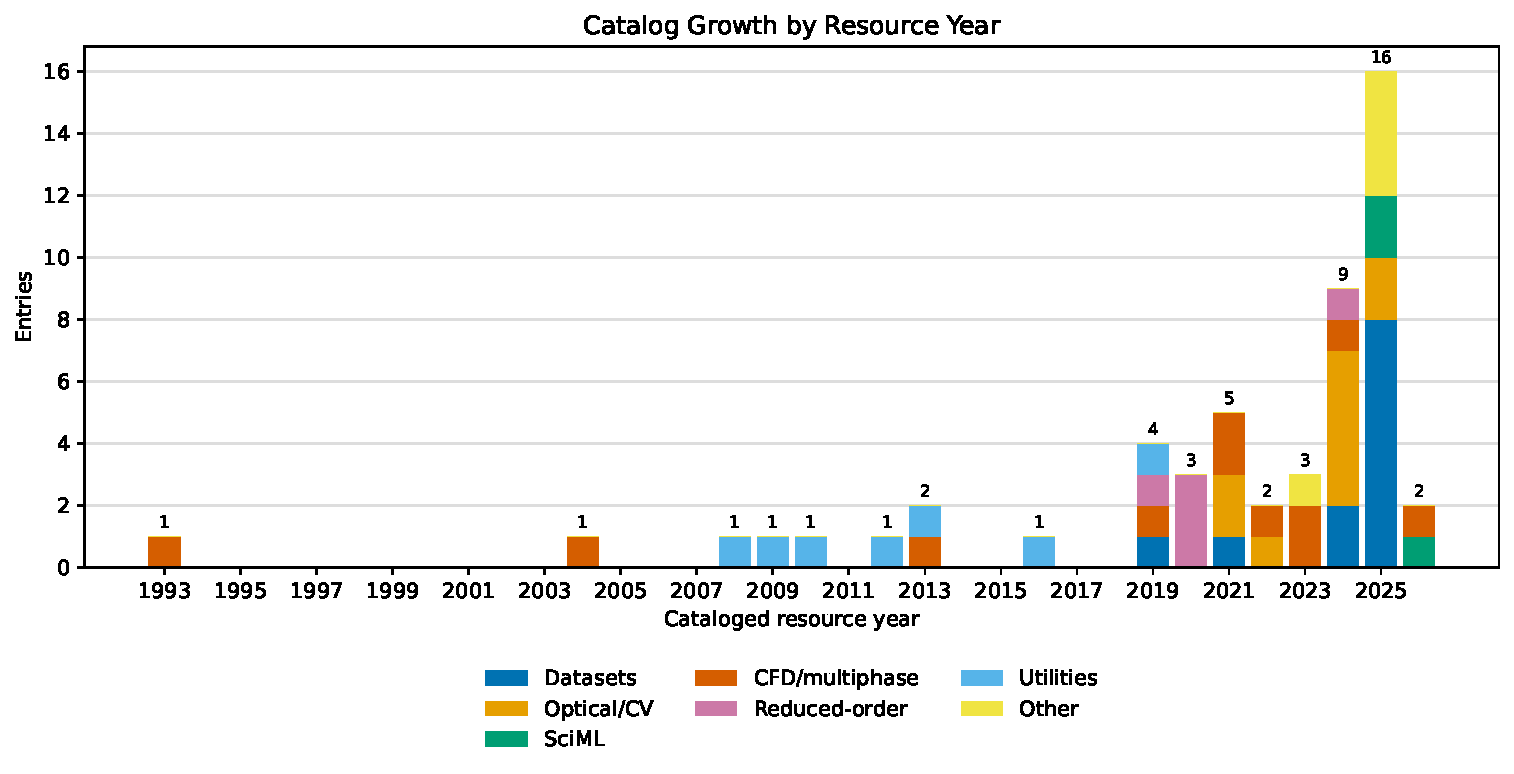
\includegraphics[width=0.95\linewidth]{figures/resource_timeline.pdf}
\caption{Catalog entries by resource year and workflow category. The year is the resource release, dataset publication, or associated publication year used for curation.}
\label{fig:timeline}
\end{figure}

The modality map in Fig.~\ref{fig:modalities} shows that the catalog is no longer just an image-processing list. Optical and video resources remain central, but several datasets combine image, acoustic, acoustic-emission, and thermal measurements. Simulation fields and reduced-order states appear in the SciML, CFD, and reduced-order groups. This modality diversity is important because modern boiling diagnostics increasingly rely on sensor fusion or cross-modal labels rather than a single camera stream. The optical/computer-vision layer is also more methodologically diverse than a flat count suggests: BubbleID focuses on pool-boiling interface dynamics \cite{dunlap2024bubbleid}, BubMask extends instance segmentation to complex gas-liquid bubbly flows \cite{kim2021bubmask}, BubbleNet targets micro-bubble flow inference with semi-physics-informed learning \cite{zhai2022bubblenet}, and FluidNexus shows how single-view videos can be lifted into multi-view fluid reconstructions and future predictions \cite{gao2025fluidnexus}. The utility layer remains essential because widely used baseline tools such as scikit-image, Trackpy, napari, Fiji, and PIVlab provide the inspection, annotation-review, centroid/linking, and flow-field extraction infrastructure that many bubble-specific models still depend on \cite{vanderwalt2014scikitimage,allan2024trackpy,sofroniew2024napari,schindelin2012fiji,thielicke2021pivlab}.

\begin{figure}[t]
\centering
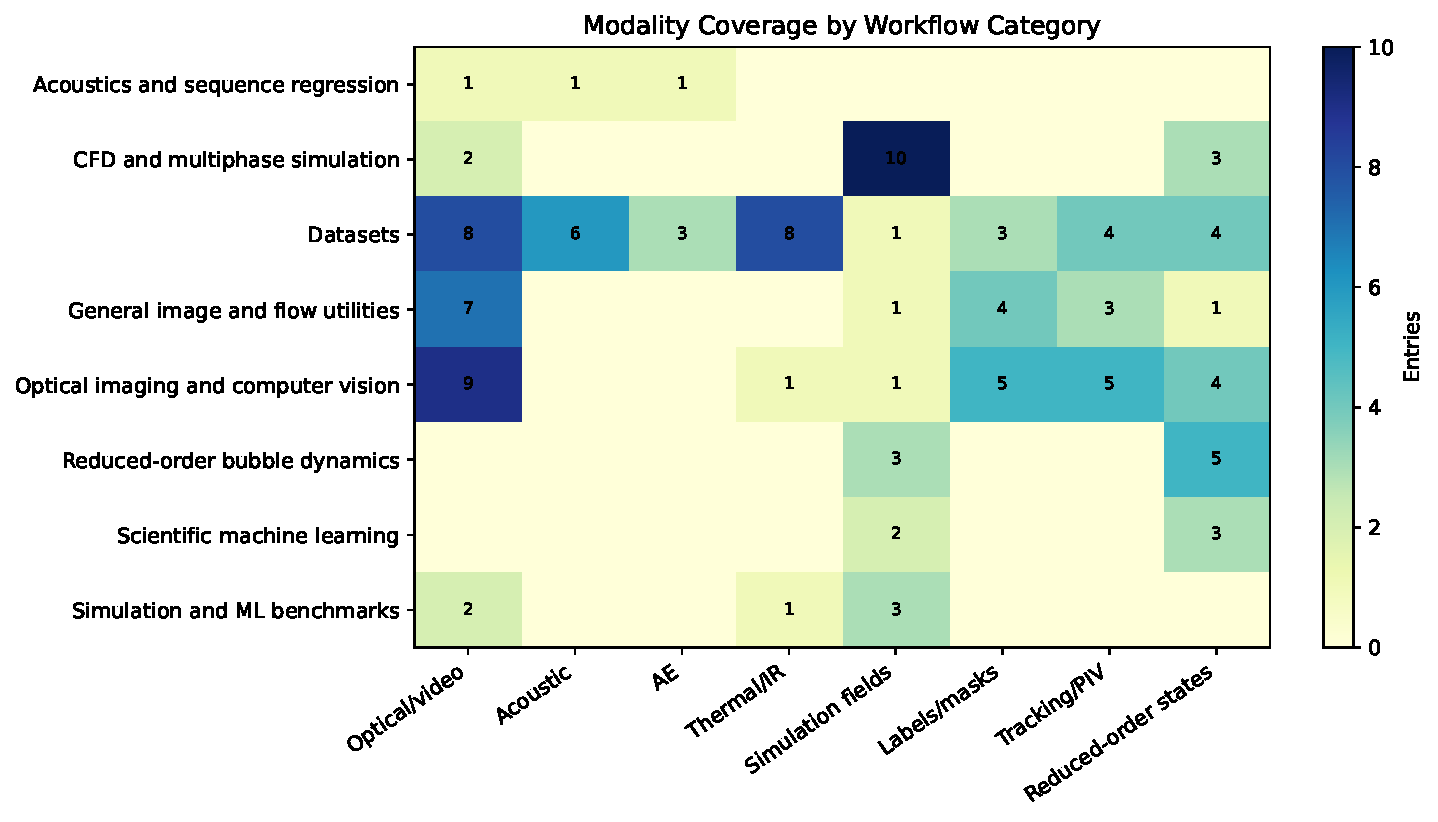
\includegraphics[width=0.95\linewidth]{figures/modality_heatmap.pdf}
\caption{Modality coverage by workflow category. A single resource can contribute to multiple modality tags.}
\label{fig:modalities}
\end{figure}

Figure~\ref{fig:evidence} shifts the emphasis from raw counts to curation quality. Several entries expose strong evidence bundles such as code plus data plus paper, but a nontrivial share still require manual license inspection or deeper source review. The metadata-coverage dashboard in the repository complements this figure by showing which workflow categories still lag in paper-link coverage, which entries expose truly open or permissive reuse terms, and which instead provide explicit but restrictive conditions such as CC BY-NC or CC BY-NC-ND. As of the June 25 pass, direct upstream license verification for BubbleNet and BubMask removes a misleading artifact in the optical/computer-vision category: that layer is now materially stronger on reuse terms than the June 24 snapshot suggested. The June 28 pass fixes a second artifact by ensuring restrictive Creative Commons terms are no longer counted as open, which matters for users who need a fast, defensible starting point rather than a broad reading list.

\begin{figure}[t]
\centering
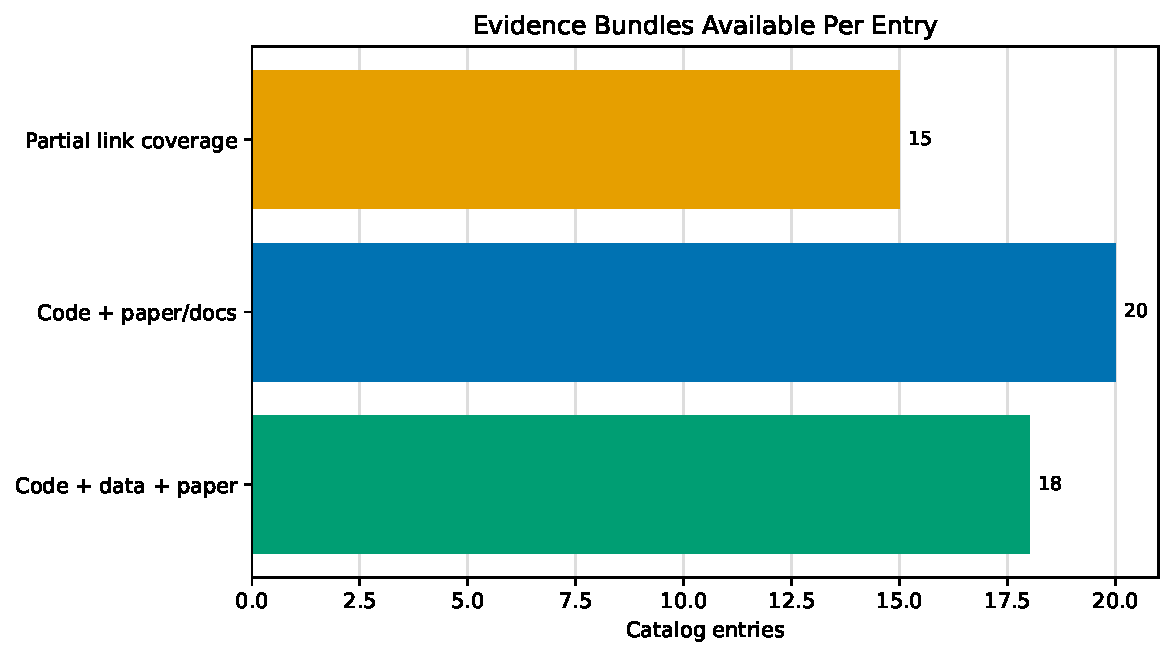
\includegraphics[width=0.86\linewidth]{figures/curation_evidence_summary.pdf}
\caption{Evidence bundles available per catalog entry. Stronger bundles are easier to reproduce, benchmark, and justify in downstream manuscripts.}
\label{fig:evidence}
\end{figure}

Figure~\ref{fig:reviewdebt} shows why repeated review comments should no longer be interpreted as a vague global metadata complaint. The remaining debt is concentrated in specific places: datasets still dominate paper-evidence and URL-discoverability limitations, reduced-order dynamics remains the weakest mixed paper-plus-license category, and CFD infrastructure has narrowed to a small residue centered on MFiX after the OpenFOAM guide pages were reinterpreted as documentation linked to licensed parent software projects rather than as standalone license-debt rows. That concentration is a more actionable maintenance signal than another flat queue of unresolved rows because it shows where a future pass should spend effort to materially improve category-level confidence. The June 26 through July 3 audits extend this logic one step further in the generated markdown outputs by ranking the remaining row-level frontier, separating `catalog backfill` from `citation discoverability` and `upstream sparsity` at the category level, and now also exposing whether a row is core to bubble and boiling workflows or merely a peripheral transfer-only asset. That extra scope signal matters because a stale immersion-cooling sharing link or a gas-solid solver metadata gap should not outrank repeated reduced-order bubble-dynamics weaknesses simply because both happen to be unresolved.

\begin{figure}[t]
\centering
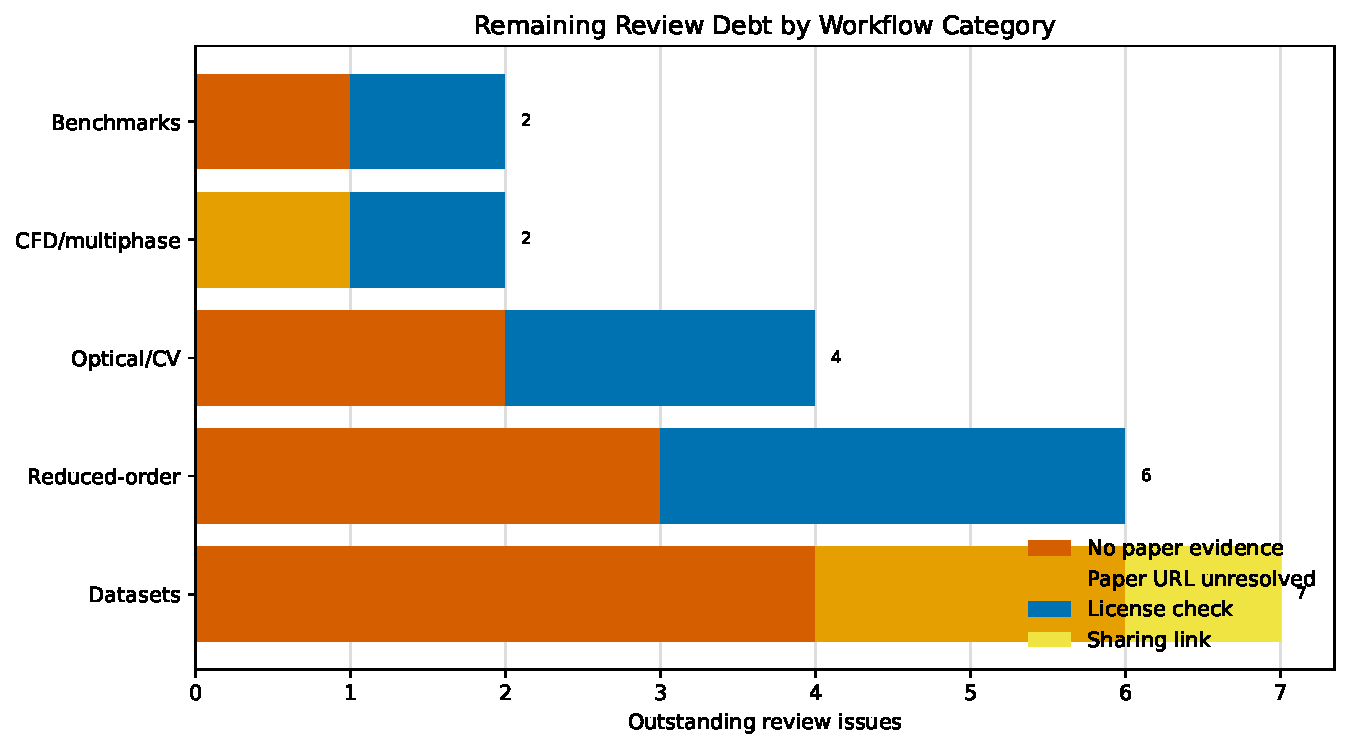
\includegraphics[width=0.9\linewidth]{figures/review_debt_by_category.pdf}
\caption{Outstanding review debt grouped by workflow category and issue type. The remaining weak spots are concentrated rather than field-wide.}
\label{fig:reviewdebt}
\end{figure}

\section{Representative User Workflows}

Table~\ref{tab:workflows} gives practical starting points. These recommendations are not universal rankings; they map common research needs to resources that are likely to be useful first stops.

\begin{table}[t]
\centering
\caption{Example workflows supported by the catalog.}
\label{tab:workflows}
\begin{tabularx}{\linewidth}{@{}lX@{}}
\toprule
Need & Suggested starting point \\
\midrule
Pool-boiling image segmentation, tracking, and interface statistics & BubbleID and the BubbleID dataset \cite{dunlap2024bubbleid}. \\
Heat-flux prediction from hydrophone, AE, or image sequences & SeqReg, hydrophone heat-flux data, and Hit2Flux-style datasets \cite{dunlap2023acoustic,dunlap2025hit2flux}. \\
High-speed-video phase segmentation across fluids & VideoSAM and its open phase-detection dataset \cite{maduabuchi2024videosam}. \\
Subcooled-flow-boiling bubble detection and thermal-hydraulic features & Zhou and co-workers' YOLO/tracking datasets and code \cite{zhou2024subcooled,zhou2025thermalhydraulic}. \\
Long-horizon SciML forecasting of boiling dynamics & BubbleML, BubbleML 2.0, Bubbleformer, and NUCLEUS \cite{hassan2023bubbleml,hassan2025bubbleformer,feeney2026nucleusmoe}. \\
Interface-resolved CFD or solver verification & Basilisk \cite{popinet2009basilisk}, Aphros, OpenFOAM \cite{jasak2007openfoam}, and Rayleigh-Plesset-style reduced-order tests. \\
Compressible bubble collapse, cavitation, or shock-bubble studies & MFC \cite{wilfong2026mfc} when compressibility or sub-grid bubble models matter. \\
\bottomrule
\end{tabularx}
\end{table}

For each workflow, the repository emphasizes validation before scale-up. In image analysis, users should inspect masks, labels, track continuity, and failure cases before generating statistics. In acoustic regression, train/test splits should separate experiments, surfaces, or fluids rather than randomly mixing windows from the same run. In CFD and SciML workflows, users should record boundary conditions, phase-change assumptions, property models, mesh or resolution studies, and physical error metrics such as heat-flux consistency or mass conservation.

\section{Maintenance Infrastructure}

The repository contains two lightweight scripts. The first, \texttt{scripts/render\_catalog.py}, validates the CSV source table and regenerates the markdown catalog, summary page, reproducibility audit, and figures. The second, \texttt{scripts/discover\_candidates.py}, uses saved GitHub queries together with manual web and archive search seeds to create a candidate report for triage without biasing discovery toward repository-hosted code alone. The project also includes a resource-suggestion issue template and a GitHub Actions workflow that validates generated files on pull requests and can run a scheduled discovery report.

This workflow is deliberately human-in-the-loop. Automatically adding resources would make the catalog noisy and could imply unearned validation. Instead, the discovery script helps maintainers notice new candidates, while the acceptance criteria require manual inspection of relevance, license, documentation quality, reproducibility artifacts, and physical-regime limits. The June 23 through June 26 maintenance passes illustrate why this matters: several recurring audit gaps were not missing because the projects lacked citations or terms, but because those details had not yet been transferred from upstream READMEs into the CSV, and the recurring reduced-order backlog shows the complementary failure mode where direct rechecks still cannot justify upgrading a row until upstream evidence genuinely exists. The targeted discovery queries now explicitly include reduced-order bubble dynamics, infrared/thermal boiling tools, and acoustic-emission boiling tools so future growth is less biased toward the already-strong optical layer.

\section{Limitations}

The catalog is not a systematic review, bibliometric database, or guarantee of correctness. It is a curated research-tool index. The counts in the figures reflect entries selected for practical reuse, so they should not be interpreted as publication rates or field-wide adoption metrics. Some entries have incomplete license information, some datasets are large or access-limited, and some code repositories are research prototypes rather than stable packages. The repository also depends on community maintenance; if source pages change, links and metadata need to be rechecked.

The most important technical limitation is transferability. A segmentation model trained on one lighting condition, heater surface, fluid, pressure, or optical path may fail on another. A boiling surrogate trained on one simulation family may extrapolate poorly outside its design space. A CFD solver example is not evidence that a new boiling case is validated. A second limitation is metadata asymmetry: some datasets expose rich README-level provenance without a stable paper URL, while some long-lived infrastructure projects expose strong community adoption but still require manual license or citation interpretation from non-DOI sources. For this reason, the catalog pairs each entry with notes on modality, workflow, and caution rather than presenting resources as interchangeable black boxes.

\section{Conclusions}

The \emph{Bubble Dynamics Research Tools} repository provides a maintainable map of open data, code, models, solvers, and utilities for bubble-dynamics research. The July 2026 snapshot contains 54 usable entries plus one name-collision guardrail and highlights a clear trend toward multimodal boiling datasets, trainable segmentation-and-tracking pipelines, acoustic and AE heat-flux models, and SciML benchmarks for long-horizon boiling forecasts. By storing catalog metadata in a structured CSV file and generating documentation and figures from that source, the repository reduces the drift that affects static awesome lists. The most useful next step is community curation: adding new resources, checking licenses and examples, and documenting validation limits as the field continues to move toward data-rich and model-assisted bubble-dynamics research.

\section*{Data and Code Availability}

The catalog, rendering scripts, figures, and this manuscript draft are available in the repository at \url{https://github.com/UARK-NED3/Bubble-Dynamics-Research-Tools}. The machine-readable source table is \texttt{data/resources.csv}.

\section*{Declaration of Generative AI and AI-Assisted Technologies}

This draft was prepared with AI-assisted writing and coding support. The catalog entries, figures, and claims should be reviewed by domain experts before submission or archival release.

\bibliographystyle{unsrt}
\bibliography{references}

\end{document}
